\documentclass[conference]{IEEEtran}
\IEEEoverridecommandlockouts
\usepackage[utf8]{inputenc}
\usepackage[T1]{fontenc}
\usepackage[spanish,es-tabla]{babel}
\usepackage{cite}
\usepackage{amsmath,amssymb,amsfonts}
\usepackage{graphicx}
\usepackage{textcomp}
\usepackage{booktabs}
\usepackage{url}
\def\BibTeX{{\rm B\kern-.05em{\sc i\kern-.025em b}\kern-.08em
    T\kern-.1667em\lower.7ex\hbox{E}\kern-.125emX}}
\def\IEEEkeywordsname{Palabras clave}
\begin{document}

\title{Detección de limones con YOLO26 y optimización bayesiana de hiperparámetros para un robot recolector}

\author{\IEEEauthorblockN{Gabriela Belén Orrego Arzamendia}
\IEEEauthorblockA{\textit{Ingeniería Mecatrónica, Facultad de Ingeniería} \\
\textit{Universidad Nacional de Asunción (FIUNA)}\\
San Lorenzo, Paraguay \\
gorrego@fiuna.edu.py}
}

\maketitle

\begin{abstract}
Este trabajo presenta un detector de limones amarillos basado en YOLO26n para el sistema de visión de un robot recolector que opera en un ambiente controlado. Se parte de un dataset público de 915 imágenes y de 50 fotos propias de un limonero en maceta, de las que se generan cuatro características por limón: tamaño, forma, color y densidad. Se entrena un modelo base por transferencia de aprendizaje desde COCO y se optimizan cinco hiperparámetros con Optuna en 12 pruebas, maximizando el mAP50-95 en validación. En las 10 fotos de test, el modelo optimizado alcanza una precisión de 0,963, un recobrado de 0,948 y un mAP50-95 de 0,729, frente a 0,960, 0,862 y 0,723 del modelo base. La mejora se concentra en el recobrado; la de mAP50-95 no es concluyente con tan pocas imágenes. El modelo falla más con limones chicos y oscuros. Además se comparan YOLO26n, YOLO11n y YOLO26s con los mismos hiperparámetros, en las fotos propias y en 100 fotos públicas apartadas del entrenamiento: las dos versiones pequeñas rinden parecido y YOLO26s ajusta mejor las cajas (mAP50-95 de 0,805 contra unos 0,75) con cuatro veces más parámetros. Se discuten las limitaciones y el trabajo futuro.
\end{abstract}

\begin{IEEEkeywords}
detección de objetos, YOLO, optimización de hiperparámetros, Optuna, visión artificial, agricultura de precisión
\end{IEEEkeywords}

\section{Introducción}
La cosecha manual de frutas es una tarea repetitiva que depende de mano de obra, y la automatización con robots requiere que el sistema de visión encuentre cada fruto entre hojas, sombras y otros frutos. La posición del fruto en la imagen es la entrada que el brazo necesita para planificar su movimiento, por lo que un detector confiable es la primera pieza de un robot recolector \cite{zhao2016}.

La detección de frutas con redes neuronales profundas es un tema activo. Sa \textit{et al.} adaptaron un detector de dos etapas a varias frutas \cite{sa2016}, Bargoti y Underwood lo aplicaron a huertos de manzanas, mangos y almendras \cite{bargoti2017} y Koirala \textit{et al.} revisaron los métodos de aprendizaje profundo para detección de frutas y estimación de rendimiento \cite{koirala2019}. La familia YOLO plantea la detección como una única regresión de cajas y clases sobre toda la imagen \cite{redmon2016}, lo que la hace adecuada para hardware limitado. La versión más reciente, YOLO26, ofrece inferencia de extremo a extremo sin supresión de no máximos y una variante \textit{nano} pensada para dispositivos de borde \cite{yolo26}. Con pocas imágenes propias, la transferencia de aprendizaje desde un modelo preentrenado \cite{pan2010} permite ajustar un detector a una clase nueva, y la búsqueda automática de hiperparámetros \cite{bergstra2011,akiba2019} evita ajustarlos a mano.

Este artículo describe el detector de limones de un robot recolector, la generación de características a partir de los datos, la optimización de hiperparámetros con Optuna y el análisis de sus errores. La parte de visión se reutiliza del proyecto grupal de la asignatura Robótica 1 (Grupo 2, FIUNA), del que la autora formó parte: de él provienen el robot, las fotos propias con sus etiquetas y la configuración del modelo base. Las contribuciones de este trabajo son la generación de características, la optimización con Optuna, la evaluación en un conjunto de test separado y el análisis de errores. El código y los resultados están disponibles en el repositorio del proyecto\footnote{\url{https://github.com/gabriela-orrego/detector-limones-yolo}}.

\section{Metodología}
\subsection{Datos}
Se usaron dos fuentes, resumidas en la Tabla~\ref{tab:datos}. La primera es un dataset público de limones en el árbol, etiquetado como segmentación (polígonos) y con tres clases: limón amarillo, limón verde y limón enfermo \cite{brinjal}. La segunda son 50 fotos de un limonero en maceta del laboratorio, sacadas con celular y etiquetadas con cajas por el grupo de Robótica \cite{limones}.

El preprocesamiento convirtió los datos en bruto a un formato único. Cada polígono se reemplazó por la caja que lo encierra; las tres clases pasaron a una sola, \textit{limón}, que corresponde a los limones amarillos, que son los que cosecha el robot; y se descartaron las 1989 imágenes del dataset público que contenían limones verdes o enfermos, porque dejarlos sin etiquetar enseñaría al modelo que un limón es fondo. Las 30 fotos propias de entrenamiento se repiten varias veces (sobremuestreo), porque son pocas frente a las del dataset público y son las más parecidas a la escena real. El conjunto de validación (10 fotos propias) sirve para elegir el mejor modelo y los hiperparámetros; el de test (10 fotos propias) no se usa hasta la evaluación final.

\begin{table}[t]
\caption{Datos utilizados tras la limpieza}
\label{tab:datos}
\centering
\small
\begin{tabular}{lccl}
\toprule
\textbf{Dataset} & \textbf{Imágenes} & \textbf{Limones} & \textbf{Uso} \\
\midrule
Público & 915 & 1315 & Entrenamiento \\
Propio, train & 30 & 175 & Entrenamiento \\
Propio, valid & 10 & 58 & Validación \\
Propio, test & 10 & 58 & Test \\
\bottomrule
\end{tabular}
\end{table}

\subsection{Características generadas}
A partir de los píxeles y de los cuatro números de cada caja (centro, ancho y alto normalizados) se calculan cuatro características por cada limón etiquetado:
\begin{itemize}
\item \textit{Tamaño}: el lado equivalente de la caja en píxeles de una imagen de 640~px, $l=640\sqrt{wh}$, donde $w$ y $h$ son el ancho y el alto normalizados. Se agrupa en chico ($l<32$), mediano ($32\le l\le 96$) y grande ($l>96$), los cortes de COCO \cite{lin2014}. Equivale a la distancia al limón.
\item \textit{Forma}: el aspecto $a=(wW)/(hH)$, con $W$ y $H$ el ancho y el alto de la imagen en píxeles. Un limón entero da un valor cercano a 1; uno tapado por hojas o cortado por el borde se aleja de 1.
\item \textit{Color}: la mediana del tono, la saturación y el brillo (HSV) en la mitad central de la caja, para no mezclar el fondo. El tono se expresa en grados.
\item \textit{Densidad}: la cantidad de limones etiquetados en la misma imagen.
\end{itemize}
Estas características no son entradas del modelo, porque YOLO aprende sus propias representaciones a partir de los píxeles. Se usan para comparar los dos datasets, para justificar los hiperparámetros de aumento de datos que se optimizan y para analizar en qué tipo de limón se equivoca el modelo. La Fig.~\ref{fig:features} compara los dos datasets: en las fotos propias los limones son más chicos (mediana de 58~px contra 124~px; el 14\,\% son grandes contra el 61\,\% del dataset público) y aparecen más juntos (mediana de 6 limones por foto contra 1). El tono es casi igual (44$^\circ$ contra 46$^\circ$), pero las fotos propias son algo más oscuras (brillo mediano de 0,78 contra 0,83). Es decir, el dataset público tiene limones grandes y aislados, y el robot verá limones chicos y en racimo.

\begin{figure}[t]
\centering
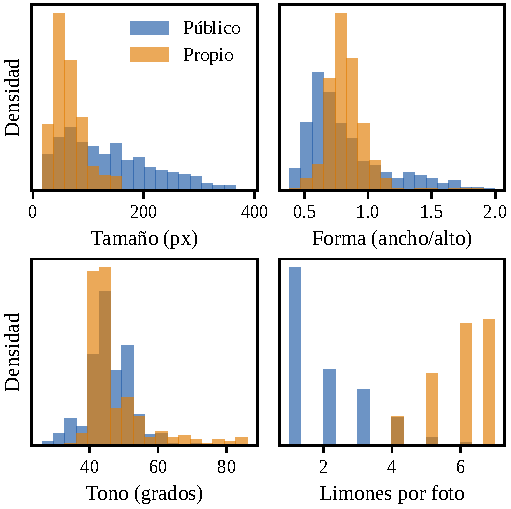
\includegraphics[width=\columnwidth]{fig_features.pdf}
\caption{Características de los limones: dataset público contra fotos propias.}
\label{fig:features}
\end{figure}

\subsection{Modelo base y optimización}
Se usó YOLO26n \cite{yolo26} con la biblioteca Ultralytics (versión 8.4.153), con 2,4 millones de parámetros. Se parte de pesos preentrenados en COCO \cite{lin2014} y se ajusta a una sola clase, con imágenes de 640~px, hasta 60 épocas y detención temprana con paciencia de 20 épocas. El optimizador es AdamW con tasa de aprendizaje inicial de 0,002, el que eligió la configuración automática de Ultralytics en el modelo base. Estos son los valores de la versión 3 del detector del grupo de Robótica.

La optimización de hiperparámetros se hizo con Optuna \cite{akiba2019} y su muestreador TPE \cite{bergstra2011}. Se eligió una búsqueda bayesiana en lugar de una grilla porque cada prueba es un entrenamiento completo: una grilla de cinco hiperparámetros con tres valores cada uno serían 243 entrenamientos. La métrica que se maximiza es el mAP50-95 sobre las 10 fotos de validación. La Tabla~\ref{tab:espacio} muestra el espacio de búsqueda. Se hicieron 12 pruebas de hasta 30 épocas, con paciencia de 10; las primeras cinco exploran el espacio (la primera usa los valores del modelo base) y las siete restantes las guía TPE. Con la mejor combinación se entrenó el modelo final durante 60 épocas, igual que el base.

\begin{table}[t]
\caption{Espacio de búsqueda y mejor combinación}
\label{tab:espacio}
\centering
\footnotesize
\setlength{\tabcolsep}{3pt}
\begin{tabular}{lccc}
\toprule
\textbf{Hiperparámetro} & \textbf{Rango} & \textbf{Base} & \textbf{Mejor} \\
\midrule
\texttt{lr0} (log) & $3\times10^{-4}$ a $10^{-2}$ & 0,002 & 0,00046 \\
\texttt{weight\_decay} (log) & $5\times10^{-5}$ a $5\times10^{-3}$ & 0,0005 & 0,00013 \\
\texttt{hsv\_h} & 0 a 0,08 & 0,015 & 0,015 \\
\texttt{scale} & 0,2 a 0,9 & 0,5 & 0,85 \\
Repeticiones fotos propias & 1, 3 o 5 & 3 & 5 \\
\bottomrule
\end{tabular}
\end{table}

\subsection{Comparación de versiones y test público}
Siguiendo las sugerencias recibidas en la presentación, se comparan tres versiones de YOLO y se agrega un test con fotos públicas. Como el entrenamiento anterior usa las 915 imágenes públicas, para este experimento se apartan 100 fotos. Las imágenes del dataset provienen de Roboflow y una misma foto original puede dar varias imágenes; por eso el sorteo (semilla 0) se hace sobre las fotos originales: se deja una imagen de cada una para el test y se excluyen del entrenamiento todas sus variantes. El test público queda con 100 imágenes y 139 limones.

Se entrenan YOLO26n, YOLO11n \cite{yolo11} y YOLO26s con los mismos datos (las imágenes públicas restantes y las 30 fotos propias repetidas cinco veces), la misma semilla, AdamW y los hiperparámetros que Optuna encontró para YOLO26n (Tabla~\ref{tab:espacio}), hasta 60 épocas con paciencia de 20. Los hiperparámetros no se reoptimizaron para cada versión. Cada modelo se evalúa en las 10 fotos propias de test y en las 100 fotos públicas apartadas. El modelo de la sección anterior se evalúa solo en las fotos propias, porque ya vio las públicas al entrenar. También se mide el tiempo de inferencia por imagen en la GPU y en la CPU de Google Colab.

\subsection{Métricas de evaluación}
Una detección es un acierto (verdadero positivo, VP) si su caja se superpone con la de un limón real aún no asignado con una intersección sobre unión $\mathrm{IoU}=|A\cap B|/|A\cup B|\ge 0,5$. Una detección sin limón real es un falso positivo (FP) y un limón real sin detectar es un falso negativo (FN). Con ellos,
\begin{equation}
P=\frac{\mathrm{VP}}{\mathrm{VP}+\mathrm{FP}},\quad R=\frac{\mathrm{VP}}{\mathrm{VP}+\mathrm{FN}},\quad F_1=\frac{2PR}{P+R},
\end{equation}
donde $P$ es la precisión y $R$ el recobrado. Además se usa el mAP50, el área bajo la curva de precisión y recobrado con umbral de IoU de 0,5 \cite{everingham2010}, y el mAP50-95, que promedia ese valor para umbrales de IoU de 0,5 a 0,95 y mide qué tan ajustadas son las cajas. El mAP50-95 es la métrica que se optimiza. El criterio de aceptación del robot es $P\ge0,80$ y $R\ge0,80$. Las matrices de confusión y los histogramas de error se calculan con un umbral de confianza fijo de 0,40. Las métricas de las tablas las calcula Ultralytics, que usa el umbral de confianza que maximiza $F_1$, por lo que el recobrado de la matriz puede diferir.

\section{Resultados}
\subsection{Búsqueda de hiperparámetros}
La Tabla~\ref{tab:pruebas} muestra las 12 pruebas y la Fig.~\ref{fig:optuna} su evolución. La prueba 11 obtuvo el mejor mAP50-95 en validación, 0,830, contra 0,756 de la prueba 0, que usa los valores base: una mejora de 0,074. Las cuatro mejores pruebas tienen una tasa de aprendizaje inicial menor que $7,5\times10^{-4}$, y las de $2\times10^{-3}$ o más dieron entre 0,751 y 0,780; es la tendencia más clara, aunque no una regla, porque la prueba 6 tiene una tasa baja y rindió 0,764. Las cuatro mejores pruebas usan un \texttt{scale} alto (0,78 a 0,87), coherente con que las fotos propias tengan limones más chicos que el dataset público (Fig.~\ref{fig:features}), y repiten 5 veces las fotos propias. Con \texttt{hsv\_h} y \texttt{weight\_decay} no se observa una tendencia con solo 12 pruebas. Como cada prueba usó una sola semilla y la validación tiene 58 limones, diferencias de 0,01 a 0,02 están dentro del ruido.

\begin{table*}[t]
\caption{Pruebas de Optuna y métricas en validación (en negrita, la mejor)}
\label{tab:pruebas}
\centering
\small
\begin{tabular}{cccccccccc}
\toprule
\textbf{Prueba} & \texttt{lr0} & \texttt{weight\_decay} & \texttt{hsv\_h} & \texttt{scale} & \textbf{Repet.} & $P$ & $R$ & mAP50 & mAP50-95 \\
\midrule
0 & 2,0$\times10^{-3}$ & 5,0$\times10^{-4}$ & 0,015 & 0,50 & 3 & 0,964 & 0,913 & 0,963 & 0,756 \\
1 & 2,1$\times10^{-3}$ & 1,3$\times10^{-3}$ & 0,048 & 0,58 & 3 & 0,973 & 0,879 & 0,973 & 0,776 \\
2 & 6,8$\times10^{-3}$ & 4,2$\times10^{-3}$ & 0,031 & 0,75 & 5 & 1,000 & 0,874 & 0,940 & 0,755 \\
3 & 3,8$\times10^{-4}$ & 7,5$\times10^{-5}$ & 0,002 & 0,78 & 5 & 0,917 & 0,956 & 0,977 & 0,801 \\
4 & 4,9$\times10^{-3}$ & 4,2$\times10^{-4}$ & 0,062 & 0,28 & 5 & 0,996 & 0,879 & 0,921 & 0,751 \\
5 & 4,7$\times10^{-4}$ & 2,1$\times10^{-4}$ & 0,014 & 0,87 & 5 & 0,982 & 0,923 & 0,982 & 0,803 \\
6 & 3,2$\times10^{-4}$ & 2,0$\times10^{-3}$ & 0,069 & 0,65 & 5 & 0,912 & 0,889 & 0,945 & 0,764 \\
7 & 4,9$\times10^{-4}$ & 1,0$\times10^{-4}$ & 0,003 & 0,36 & 5 & 1,000 & 0,906 & 0,977 & 0,788 \\
8 & 3,5$\times10^{-3}$ & 6,0$\times10^{-5}$ & 0,040 & 0,76 & 5 & 1,000 & 0,890 & 0,959 & 0,779 \\
9 & 1,4$\times10^{-3}$ & 4,4$\times10^{-4}$ & 0,057 & 0,79 & 5 & 0,931 & 0,948 & 0,974 & 0,774 \\
10 & 7,3$\times10^{-4}$ & 3,4$\times10^{-3}$ & 0,030 & 0,85 & 5 & 0,991 & 0,931 & 0,973 & 0,789 \\
\textbf{11} & \textbf{4,6$\times10^{-4}$} & \textbf{1,3$\times10^{-4}$} & \textbf{0,015} & \textbf{0,85} & \textbf{5} & \textbf{0,971} & \textbf{0,983} & \textbf{0,992} & \textbf{0,830} \\
\bottomrule
\end{tabular}
\end{table*}

\begin{figure}[t]
\centering
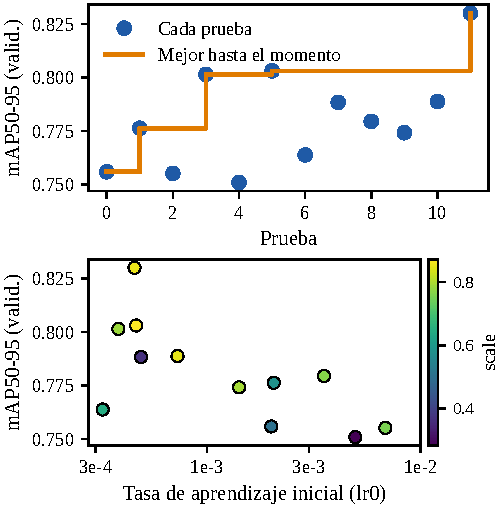
\includegraphics[width=\columnwidth]{fig_optuna.pdf}
\caption{Búsqueda con Optuna. Arriba, el mAP50-95 de cada prueba y el mejor acumulado. Abajo, el mAP50-95 según la tasa de aprendizaje inicial; el color indica \texttt{scale}.}
\label{fig:optuna}
\end{figure}

\subsection{Entrenamiento y convergencia}
La Fig.~\ref{fig:curvas} muestra el entrenamiento final. El modelo optimizado entrenó las 60 épocas y su mejor época fue la 56; las pérdidas de entrenamiento y de validación bajaron hasta el final, sin señal clara de sobreajuste. En el modelo base, el mAP50-95 de validación dejó de mejorar en la época 31 y el entrenamiento se detuvo en la 51. En validación, el mAP50-95 pasó de 0,778 (base) a 0,811 (optimizado). El 0,830 de la búsqueda es algo optimista, porque se eligió justamente por ese valor.

\begin{figure}[t]
\centering
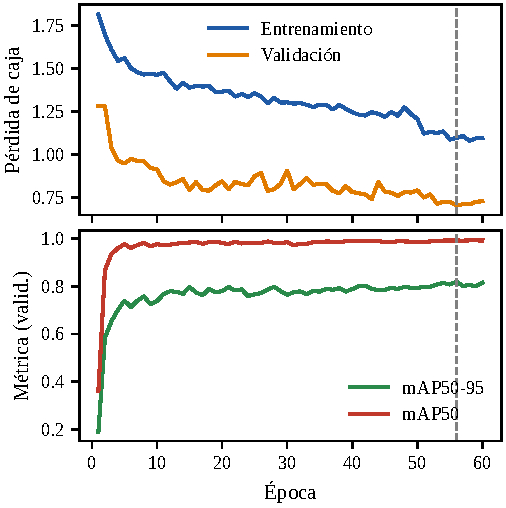
\includegraphics[width=\columnwidth]{fig_curvas.pdf}
\caption{Entrenamiento del modelo optimizado. Arriba, la pérdida de caja. Abajo, las métricas en validación. La línea punteada marca la mejor época.}
\label{fig:curvas}
\end{figure}

\subsection{Comparación en test}
La Tabla~\ref{tab:comparacion} compara los dos modelos. Las 10 fotos de test, con 58 limones, no se usaron para entrenar ni para elegir hiperparámetros, por lo que son la medida más honesta. El modelo optimizado cumple el criterio de $P$ y $R$ $\ge0,80$ y mejora sobre todo el recobrado, de 0,862 a 0,948. La diferencia en mAP50-95 es de 0,006 (0,723 a 0,729), que con 58 limones no es una diferencia confiable. Con la validación incluida (20 fotos, 116 limones) los valores del optimizado son $P=0,956$, $R=0,966$ y mAP50-95 de 0,762, contra 0,929, 0,922 y 0,746 del base; esa cifra es optimista porque la validación se usó para elegir el modelo. La inferencia tarda 9,5~ms por imagen en una GPU T4.

\begin{table}[t]
\caption{Comparación de modelos sobre las 10 fotos de test}
\label{tab:comparacion}
\centering
\small
\begin{tabular}{lccccc}
\toprule
\textbf{Modelo} & $P$ & $R$ & $F_1$ & mAP50 & mAP50-95 \\
\midrule
Base & 0,960 & 0,862 & 0,908 & 0,938 & 0,723 \\
Optimizado & \textbf{0,963} & \textbf{0,948} & \textbf{0,956} & \textbf{0,967} & \textbf{0,729} \\
\bottomrule
\end{tabular}
\end{table}

\subsection{Comparación de versiones de YOLO}
La Tabla~\ref{tab:versiones} y la Fig.~\ref{fig:versiones} muestran los resultados. En las fotos propias, las tres versiones encuentran casi los mismos limones (mAP50 de 0,959 a 0,960; recobrado de 0,925 a 0,944, una diferencia de un limón sobre 58). YOLO26s tiene el mAP50-95 más alto (0,805 contra 0,754 y 0,749), lo que indica cajas más ajustadas a cada limón y no más limones detectados. Esta ventaja es una pista y no una prueba: hay una sola semilla, el test tiene 58 limones y los hiperparámetros están afinados para YOLO26n. YOLO26n y YOLO11n quedan prácticamente empatados. El YOLO26n entrenado sin las 100 fotos públicas rinde parecido al de la sección anterior en las fotos propias (mAP50-95 de 0,754 contra 0,729), así que apartarlas no empeoró el modelo.

\begin{table*}[t]
\caption{Versiones de YOLO con los mismos datos e hiperparámetros. Test propio: 10 fotos, 58 limones. Test público: 100 fotos apartadas, 139 limones. Los parámetros se cuentan antes de fusionar capas.}
\label{tab:versiones}
\centering
\small
\begin{tabular}{lcccccccc}
\toprule
& & \multicolumn{3}{c}{\textbf{Test propio}} & \multicolumn{3}{c}{\textbf{Test público}} & \\
\cmidrule(lr){3-5}\cmidrule(lr){6-8}
\textbf{Modelo} & \textbf{Parám. (M)} & $P$ & $R$ & mAP50-95 & $P$ & $R$ & mAP50-95 & \textbf{Archivo (MB)} \\
\midrule
YOLO26n (sección anterior) & 2,5 & 0,963 & 0,948 & 0,729 & -- & -- & -- & 5,4 \\
YOLO26n (sin las 100 fotos) & 2,5 & 0,946 & 0,931 & 0,754 & 0,632 & 0,544 & 0,382 & 5,4 \\
YOLO11n & 2,6 & 0,947 & 0,925 & 0,749 & 0,603 & 0,622 & 0,382 & 5,5 \\
YOLO26s & 9,95 & 0,948 & 0,944 & \textbf{0,805} & 0,528 & 0,719 & 0,367 & 20,3 \\
\bottomrule
\end{tabular}
\end{table*}

\begin{figure}[t]
\centering
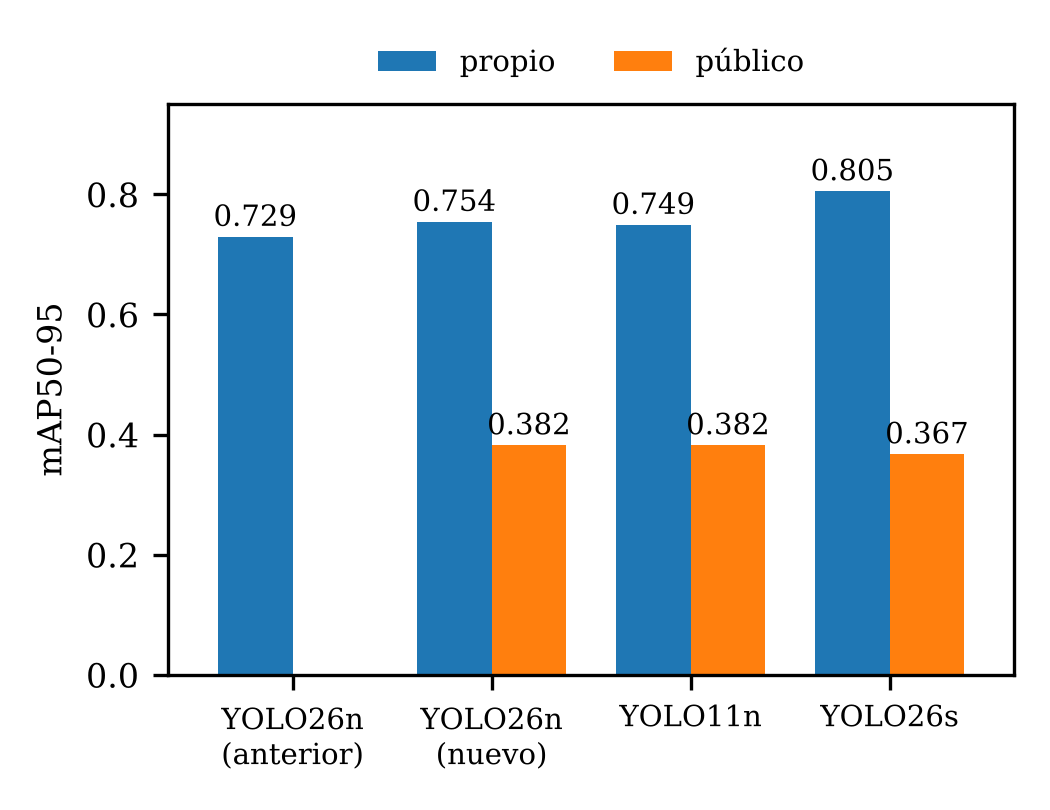
\includegraphics[width=\columnwidth]{fig_versiones.png}
\caption{mAP50-95 de cada versión en los dos conjuntos de test. «Anterior» es el modelo de la sección anterior, que no se evalúa en el test público porque ya vio esas fotos.}
\label{fig:versiones}
\end{figure}

En las 100 fotos públicas las tres versiones dan entre 0,367 y 0,382 de mAP50-95, sin diferencias que las separen. Estos valores son más bajos que los de las fotos propias y no son comparables con ellos: los dos conjuntos tienen fotos y etiquetado distintos. Una causa probable, que no se verificó, es que el dataset público tenga limones sin etiquetar, que se cuentan como falsos positivos.

Respecto del costo, YOLO26s tiene 9,95 millones de parámetros y su archivo pesa 20,3~MB, cuatro veces más que las versiones pequeñas. En la GPU de Colab las tres tardan entre 8,6 y 10,2~ms por imagen; en la CPU, YOLO26s tardó más del doble. Las mediciones en CPU variaron mucho entre corridas (el mismo YOLO26n dio 79 y 147~ms) y no se midió la velocidad en la Raspberry Pi 5, que es la que importa para el robot.

\subsection{Predicciones y análisis de errores}
La Fig.~\ref{fig:pred} muestra predicciones sobre fotos de test. La matriz de confusión de la Fig.~\ref{fig:matriz}, calculada sobre las 20 fotos de validación y test (116 limones) con un umbral de confianza de 0,40, tiene 103 aciertos, 13 limones no detectados y 4 detecciones de más; con ese umbral fijo el recobrado es 0,888. Los histogramas de la Fig.~\ref{fig:errores} muestran que las cajas están bien ajustadas (IoU medio de 0,89 y error mediano del centro de 2,4\,\% del lado del limón), que los falsos positivos son pocos y de confianza media, y que el modelo tiende a contar de menos: en 8 de las 20 fotos detecta un limón menos y en 10 el conteo es exacto.

\begin{figure}[t]
\centering
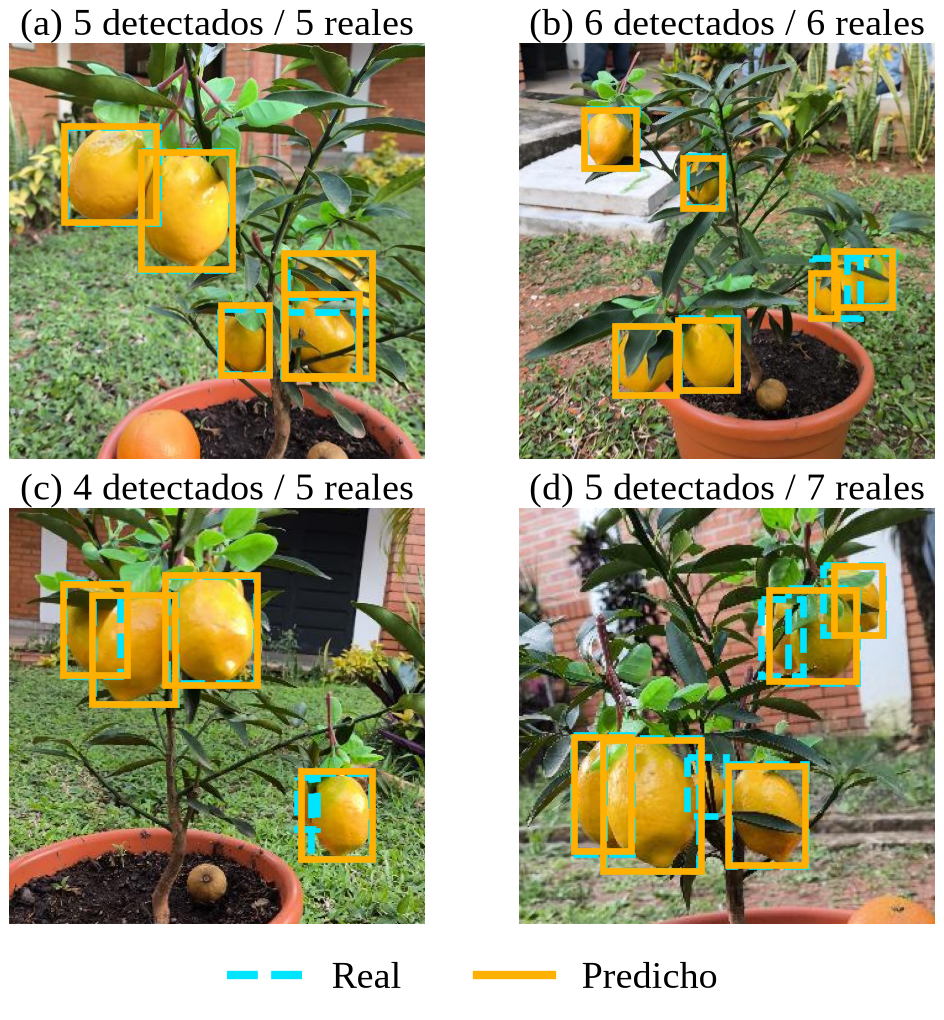
\includegraphics[width=\columnwidth]{fig_predicciones.png}
\caption{Predicciones del modelo optimizado (naranja) y limones reales (celeste) en fotos de test. El título de cada foto indica detectados y reales.}
\label{fig:pred}
\end{figure}

\begin{figure}[t]
\centering
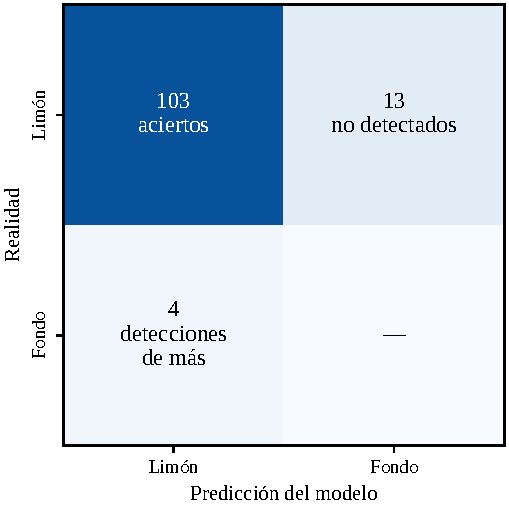
\includegraphics[width=0.85\columnwidth]{fig_matriz.pdf}
\caption{Matriz de confusión del modelo optimizado en 20 fotos (validación y test), con umbral de confianza de 0,40.}
\label{fig:matriz}
\end{figure}

\begin{figure}[t]
\centering
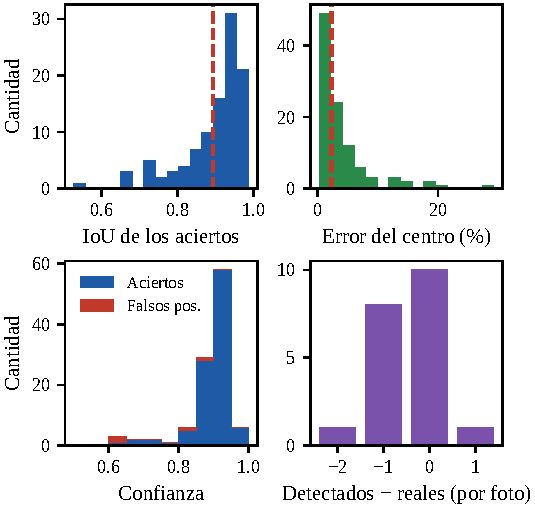
\includegraphics[width=\columnwidth]{fig_errores.pdf}
\caption{Errores del modelo optimizado. Arriba, el IoU y el error del centro de los aciertos (línea roja: media y mediana). Abajo, la confianza de aciertos y falsos positivos, y el error de conteo por foto.}
\label{fig:errores}
\end{figure}

La Tabla~\ref{tab:feature} cruza los limones reales con las características de la Sección II-B. El recobrado es menor en los limones chicos (0,667, con solo 6 casos), en los oscuros (0,789) y en las fotos de 5 o 6 limones (0,863), y mayor en los limones claros (0,937) y grandes (0,941). Con pocos casos por grupo, estos porcentajes son orientativos.

\begin{table}[t]
\caption{Recobrado del modelo optimizado según las características del limón (20 fotos)}
\label{tab:feature}
\centering
\small
\begin{tabular}{llcc}
\toprule
\textbf{Característica} & \textbf{Grupo} & \textbf{Limones} & $R$ \\
\midrule
Tamaño & chico & 6 & 0,667 \\
 & mediano & 93 & 0,892 \\
 & grande & 17 & 0,941 \\
Brillo & oscuro & 19 & 0,789 \\
 & medio & 34 & 0,853 \\
 & claro & 63 & 0,937 \\
Limones por foto & hasta 4 & 8 & 1,000 \\
 & 5 o 6 & 73 & 0,863 \\
 & 7 o más & 35 & 0,914 \\
\bottomrule
\end{tabular}
\end{table}

\section{Conclusiones}
Se desarrolló un detector de limones amarillos con YOLO26n y se lo optimizó con Optuna. En las fotos de test alcanza una precisión de 0,963 y un recobrado de 0,948, por lo que cumple el criterio de 0,80 del robot. La optimización mejoró el recobrado de 0,862 a 0,948; la mejora del mAP50-95 en test, de 0,006, no es concluyente. Las cajas son precisas y el modelo falla sobre todo con limones chicos, oscuros y en racimos de 5 o 6, donde suele contar un limón de menos.

Al comparar tres versiones de YOLO con los mismos datos e hiperparámetros, YOLO26n y YOLO11n rinden parecido en las fotos propias y en 100 fotos públicas apartadas. YOLO26s ajusta mejor las cajas en las fotos propias (mAP50-95 de 0,805 contra unos 0,75) a cambio de cuatro veces más parámetros; la diferencia es una pista y no una prueba. Con estos resultados no se puede afirmar que YOLO26n sea la mejor versión: se lo prefiere por ser mucho más liviano para la Raspberry Pi, algo que falta comprobar midiendo en el robot.

Las limitaciones son varias. El test tiene 10 fotos del mismo árbol y del mismo día que las de entrenamiento, así que las métricas son optimistas y varían mucho. Las fotos son de celular y el robot usa otras cámaras. La búsqueda tiene solo 12 pruebas con una semilla cada una, y la comparación de versiones usa los hiperparámetros afinados para YOLO26n. El dataset público parece incluir imágenes ilustradas o generadas, que se usaron solo para entrenar. Por último, el detector solo sirve para limones amarillos en un ambiente controlado, un limonero en maceta.

Como trabajo futuro se propone reunir fotos con la cámara del robot y con distinta iluminación, usar un conjunto de test más grande y varias semillas para medir mejor las diferencias, optimizar cada versión de YOLO por separado, incluir limones verdes y enfermos, e integrar el detector con el brazo midiendo el tiempo de respuesta en el hardware del robot.

\section*{Agradecimientos}
La autora agradece a sus compañeros del Grupo 2 de Robótica 1, con quienes se desarrolló el proyecto original del que proviene la parte de visión, y a los profesores de la asignatura Inteligencia Artificial, Dr. Diego Stalder e Ing. Enrique Paiva.

\begin{thebibliography}{00}
\bibitem{zhao2016} Y. Zhao, L. Gong, Y. Huang, and C. Liu, ``A review of key techniques of vision-based control for harvesting robot,'' \textit{Comput. Electron. Agric.}, vol. 127, pp. 311--323, 2016.
\bibitem{sa2016} I. Sa, Z. Ge, F. Dayoub, B. Upcroft, T. Perez, and C. McCool, ``DeepFruits: A fruit detection system using deep neural networks,'' \textit{Sensors}, vol. 16, no. 8, p. 1222, 2016.
\bibitem{bargoti2017} S. Bargoti and J. Underwood, ``Deep fruit detection in orchards,'' in \textit{Proc. IEEE Int. Conf. Robot. Autom. (ICRA)}, 2017, pp. 3626--3633.
\bibitem{koirala2019} A. Koirala, K. B. Walsh, Z. Wang, and C. McCarthy, ``Deep learning -- Method overview and review of use for fruit detection and yield estimation,'' \textit{Comput. Electron. Agric.}, vol. 162, pp. 219--234, 2019.
\bibitem{redmon2016} J. Redmon, S. Divvala, R. Girshick, and A. Farhadi, ``You only look once: Unified, real-time object detection,'' in \textit{Proc. IEEE Conf. Comput. Vis. Pattern Recognit. (CVPR)}, 2016, pp. 779--788.
\bibitem{yolo26} Ultralytics, ``YOLO26,'' Ultralytics Docs. [Online]. Available: \url{https://docs.ultralytics.com/models/yolo26/}
\bibitem{yolo11} Ultralytics, ``YOLO11,'' Ultralytics Docs. [Online]. Available: \url{https://docs.ultralytics.com/models/yolo11/}
\bibitem{pan2010} S. J. Pan and Q. Yang, ``A survey on transfer learning,'' \textit{IEEE Trans. Knowl. Data Eng.}, vol. 22, no. 10, pp. 1345--1359, Oct. 2010.
\bibitem{bergstra2011} J. Bergstra, R. Bardenet, Y. Bengio, and B. K\'egl, ``Algorithms for hyper-parameter optimization,'' in \textit{Adv. Neural Inf. Process. Syst. (NIPS)}, vol. 24, 2011, pp. 2546--2554.
\bibitem{akiba2019} T. Akiba, S. Sano, T. Yanase, T. Ohta, and M. Koyama, ``Optuna: A next-generation hyperparameter optimization framework,'' in \textit{Proc. 25th ACM SIGKDD Int. Conf. Knowl. Discovery Data Mining}, 2019, pp. 2623--2631.
\bibitem{lin2014} T.-Y. Lin \textit{et al.}, ``Microsoft COCO: Common objects in context,'' in \textit{Proc. Eur. Conf. Comput. Vis. (ECCV)}, 2014, pp. 740--755.
\bibitem{everingham2010} M. Everingham, L. Van Gool, C. K. I. Williams, J. Winn, and A. Zisserman, ``The PASCAL visual object classes (VOC) challenge,'' \textit{Int. J. Comput. Vis.}, vol. 88, no. 2, pp. 303--338, 2010.
\bibitem{brinjal} brinjalproject, ``lemons-segmentation (version 5),'' Roboflow Universe. [Online]. Available: \url{https://universe.roboflow.com/brinjalproject/lemons-segmentation}
\bibitem{limones} Grupo 2, Robótica, FIUNA, ``limones-amarillos (version 3),'' Roboflow Universe, CC BY 4.0. [Online]. Available: \url{https://universe.roboflow.com/hectors-workspace-e5dhh/limones-amarillos}
\end{thebibliography}

\end{document}
